\part{Sicurezza fisica \& del personale}
\label{SFDP}
\chapter{Difesa in profondità}

La difesa in profondità serve per proteggersi quando un livello di sicurezza 
viene superato. Questo tipo di difesa è possibile immaginarsela come gli strati 
di una cipolla. Dal punto di vista della sicurezza fisica questo si riassume in:
\begin{itemize}
\item Cancelli
\item Bidoni (quelli che si alzano nella strada per intenderci) automatici
\item Staccionate
\end{itemize}

È importante attrezzarsi anche per difendersi da eventi che possono accadere 
all'interno dell'azienda, come può essere ad esempio un incendio.

\section{Tipologie di controlli}

Le diverse tipologie di controlli sono concentriche, a difficoltà incrementanti e 
indipendenti. Questi tipi di controlli possono essere \textbf{preventivi}, 
\textbf{reattivi} e \textbf{correttivi}.

Una lista di controlli (a partire dalla parte più ``concentrica'' per muoversi 
verso quella più esterna) sono:

\todo{Traduci i punti seguenti } %Qualcuno lo traduce plis? Non avevo voglia
\begin{itemize}
\item Postazione di lavoro chiusa (Locked work stations)
\item Videocamere e sistema di allarme
\item Bonded personnel Controlled visitor access: personale ristretto 
nell'accesso
\item Security Guards, manual logging \& photo ID badges
\item Controlled single entry point \& barred windows
\item Non pubblicizzare l'ubicazione di strutture (\textit{facilities})
sensibili
\end{itemize}


Un buon consiglio è avere un numero di accessi al locale ridotto. Questo però 
non è sempre possibile, in quanto in una \textit{facility} grossa potrebbero 
esserci norme di sicurezza da seguire.

Anche dal punto di vista di riconoscimento del personale, una buona pratica è 
far indossare il badge al personale.

Ognuna delle misure esposte prima hanno un costo, e di solito che è grande, e 
possono portare a problemi. Per esempio, le registrazioni dovrebbero essere 
anche salvate in postazioni sicure in quanto potrebbero essere soggette a furti.

Quanto spenderci e quanto investire è una questione quindi a cui è difficile 
rispondere.

\section{Sicurezza fisica}
\label{SFDP:fisica}
\subsection{Protezione dalla potenza}

Classificazione in funzione del fenomeno negativo che si verifica:
\begin{itemize}
\item Surge, spikes and sags: qualcuno ha collegato un dispositivo alla rete che 
ha causato un sovraccarico nella rete causando picchi (positivi e negativi).
\item Blackout
\item Brownout: i livelli di corrente dichiarati non sono quelli effettivi sulla 
rete
\item EMI (Electromagnetic Interference): dispositivi elettrici che generano 
effetti parassitari su dispositivi terzi
\end{itemize}

I dispositivi di protezione dipendono dalla durata del fenomeno, per breve 
durata bastano i surge protector, per durata minore di 30 min si utilizza un UPS 
(universal power supply); per periodi più lunghi si usa un generatore 
alternativo di corrente. I generatori possono arrivare anche a costare milioni 
di euro.

\subsection{Equipaggiamento della computer room}

\begin{itemize}
\item Rilevatore d'acqua (a livello del pavimento)
\item Estintori
\item Allarme antincendio manuale
\item Rilevatori di fumo (in alto e in basso)
\item Switch di spegnimento d'emergenza
\end{itemize}

\subsection{Ambiente IPF}

Una sala di calcolo non va messa nei piani alti in quanto potrebbe essere 
soggetta a fulmini e a intemperie, e neanche al piano base in quanto è soggetta 
ad allagamenti. Quindi un buon posizionamento è a metà della costruzione. È 
anche importante che ci siano delle porte taglia fuoco.

\subsubsection{Sistema per la soppressione dei fuochi}

Questi sistemi possono essere:
\begin{itemize}
\item Acqua
\begin{itemize}
\item Caricato: ovvero gli estintori sono caricati, e hanno l'attivazione 
immediata. Lo svantaggio è che essendo sempre caricati potrebbero costituire un 
problema
\item Secchi
\end{itemize}
\begin{itemize}
\item Gas
\begin{itemize}
\item Pericolosi (che possono essere Halon e Anidride Carbonica)
\item Amici dell'ambiente, che non spengono veramente il fuoco, ma riducono le 
capacità ignifughe (FM-200 e Argonite)
\end{itemize}
\end{itemize}
\end{itemize}

\subsection{Sistemi di chiusura}

Esistono diversi modi di chiusura dei sistemi, che possono richiedere dalla 
autenticazione biometrica per essere sbloccati per finire fino ad una semplice 
porta elettronica.

Molti di questi sistemi sono elettrici però, ed è quindi importante che i 
meccanismi siano \textit{fail-safe}: ovvero che in mancanza della corrente 
elettrica la porta deve rimanere porta. Proprio per questo gli attaccanti 
potrebbero sfruttare ciò per guadagnare l'accesso.

\subsubsection{Porta dell'uomo morto}

Questa tecnica si basa sul \textit{piggybacking}. Per risolvere questo problema 
basta aggiungere due sistemi di entrata, in maniera tale che venga evitata 
quindi l'accesso per \textit{piggyback} di una persona.


\subsection{Computer nei luoghi pubblici}

Protezioni logiche:
\begin{itemize}
\item Imaged computers
\item Antivirus e antispyware
\item Filtri web
\item Login/password
\item Protezione firewall dal resto dell'organizzazione
\end{itemize}

Protezioni fisiche: lucchetto sul case, dispositivo della kensington per i 
laptop. Anche le etichette con il codice è meglio scriverle nello chassis del 
laptop piuttosto che usare una etichetta.

%ENGRAVE = INCIDERE
\subsection{Modile computing}

\begin{itemize}
\item Incisione del numero seriale sul laptop
\item Backup dei dati critici e sensibili
\item Criptare i dati sensibili
\item Proteggere i file importanti con password individuali
\item Individuare il responsabile del furto e segnalarlo
\end{itemize}


\subsection{Sicurezza dei dispositivi}

Le porte USB e le entrate Flash devono essere bandite o disabilitate dal 
computer, oppure è necessario eseguire una crittografia di tutti i dati.


\subsection{Criticality Table}

\begin{figure}[H]
 \centering
 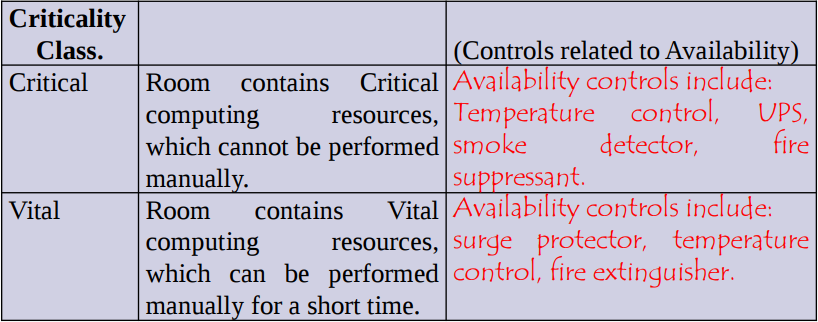
\includegraphics[width=\textwidth]{criticality-table}
\end{figure}

\subsection{Physical Security Map}
\begin{figure}[H]
 \centering
 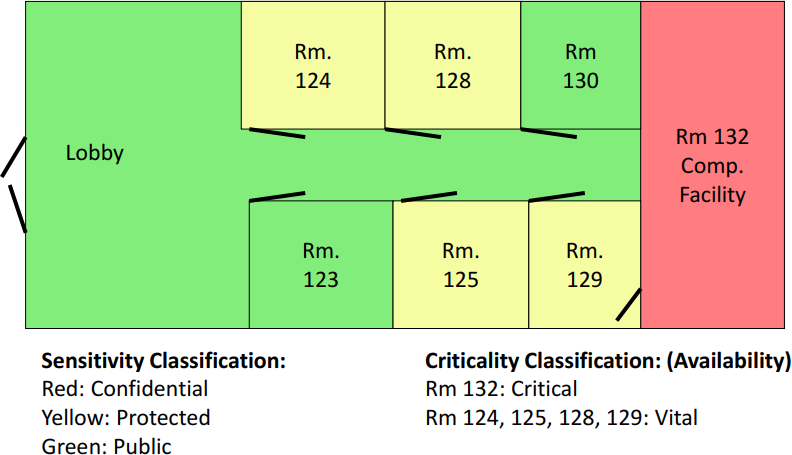
\includegraphics[width=\textwidth]{physical-security-map}
\end{figure}

\subsection{Riassunto di sicurezza fisica}

Controllo dell'accesso fisico

Controlli ambientali

Fire suppressant != Fire estinguisher

Procedure di sicurezza
\todo{copia liste}

\subsection{Esercizi}

Gli esercizi sono dispnibili nella sezione \ref{esSFDP:fisica}

\section{Sicurezza del personale}

\subsection{Consapevolezza della sicurezza \& Training}

Il training copre quello che ci si aspetta dagli impiegati?

Il training può essere implementato come: orientamento dei nuovi impiegati, 
newsletter interna alla compagnia e determinare l'efficacia intervistando gli 
impiegati.


\subsubsection{Awareness Function: types of security training}

Awareness: crea nel personale una sensibilità nei confronti di problemi di 
sicurezza.

Training: skill necessarie per una posizione particolare.

Education: skills di alto livello.
